%% LaTeX2e class for student theses
%% sections/content.tex
%% 
%% Karlsruhe Institute of Technology
%% Institute for Program Structures and Data Organization
%% Chair for Software Design and Quality (SDQ)
%%
%% Dr.-Ing. Erik Burger
%% burger@kit.edu
%%
%% Version 1.1, 2014-11-21

%To be able to reference labels in other file
\externaldocument{introduction}
\externaldocument{appendix}


\chapter{Experimental Setup}
\label{ch:LITasks}

This chapter lays out the experimental setup used in this thesis. While Language Identification is applicable in many different scenarios, here the focus lies on trying to establish a low-latency online approach for recognizing the spoken language in a university-lecture environment. Because finding a suitable test setup for online data retrieval is hard, the data used was cut to short lengths to make an evaluation as to correctness of the recognition possible in an ''online-like'' scenario. 

This means that the output of the net is evaluated after short samples of speech and therefore can be seen as indicative of online performance of the net in the lecture translator.

This chapter introduces our experimental setup as well as the data sets the experiments were conducted on.

\section{General Setup}
\label{sec:LITasks:GS}

Many different tools exist for deep learning, the most acclaimed being Tensorflow~\cite{DBLP:journals/corr/AbadiABBCCCDDDG16}, DL4J/ND4j\footnote{DL4J:~\url{https://deeplearning4j.org/index.html}} and Theano~\cite{bergstra2011theano}. Pre-existing work on Language Identification, or rather Language Feature Vector Extraction using a LID Network in~\cite{Mueller2016b}, used a python wrapper around Theano for training, that was developed by Jonas Gehring~\cite{gehringMA}. This thesis continues the use of this wrapper for the training of our DNNs. The basic layout of the network used and improved upon by this thesis were input vectors from a multilingual ASR net, further explained in Sec.~\ref{sec:FP:FA}, which we used to generate Bottleneck Features with 966 coefficients. The LID network introduced in the following chapters then uses these BNF vectors to classify the audio input into a language. Different Network Structures and types (DNNs/RNNs) were used that will be further explained in Ch.~\ref{ch:LIDNetwork}. 

As detl does not provide support for RNNs we used Lasagne~\footnote{Lasagne: \url{https://lasagne.readthedocs.io/en/latest/}}, another wrapper around theano, as the framework for our RNN training.


\section{Euronews 2014}
\label{sec:LITasks:Euronews}


The first data set used, was retrieved from Euronews \footnote{Euronews: http://www.euronews.com/} 2014. Euronews is a TV channel that is broadcast in 13 different languages simultaneously both on TV and over the Web and is semi-automatically transcribed. The data corpus includes 10 languages (Arabian, German, Spanish, French, Italian, Polish, Portuguese, Russian, Turkish and English) with around 72 hours of data per language provided overall, meaning the corpus had a total length of around 720 hours of audio data. This data was taken both from online video and recordings of the transmissions as described in \cite{gretter2014euronews}.

For the purposes of this work we then broke this corpus down further into a more manageable size as to make the feedback-cycle faster, while still keeping the corpus big enough to make results comparable to performance with the full corpus. Later, we then used the full data set to compare results between the smaller and bigger sets.

The corpus was broken down to a per-speaker-basis based on its automatic transcriptions. From this data we took a sample of a random 10.000 speakers, while making sure the total length of samples for each language were roughly the same. Details of this breakdown can be seen in table ~\ref{tab:spkData}.

\begin{table}[h!]
\label{tab:spkData}
\centering
\begin{tabular}{| l | c | r | }
	\hline
	\textbf{Language} & \textbf{Number of Speakers} & \textbf{Combined Length} \\
	\hline
	Arabian & 1055 & 16.76 h \\
	German & 928 & 18.80 h \\
	Spanish & 932 & 18.78 h \\
	French & 1016 & 18.67 h \\  
	Italian & 935 & 19.00 h \\  
	Polish & 1229 & 18.30 h \\ 
	Portuguese & 1062 & 16.19 h \\ 
	Russian & 958 & 18.66 h \\ 
	Turkish & 957 & 18.61 h \\  
	English & 928 & 18.54 h \\ 
	\hline
	\textbf{Overall} & 10000 & 182.31 h\\
	\hline
	
\end{tabular}
\caption{The euronews corpus speaker breakdown used for most experiments with total utterances length.}
\end{table}

\begin{table}[h!]
\label{tab:spkSplit}
\centering
\begin{tabular}{| l | c | r | }
	\hline
	\textbf{Set} & \textbf{Number of Speakers} & \textbf{Combined Length} \\
	\hline
	Train &  8000 & 149.76 h \\
	Development & 1000 & 19.46 h \\
	Test & 1000 & 19.29 h \\
	\hline
\end{tabular}
\caption{The Euronews corpus breakdown into the three data sets.}
\end{table}

The speaker list was then split into three smaller datasets: the train set, development set and test set using the common Simple Random Sampling. The sizes were \(80\%\) allocated to the train set, and \(10\%\) for both the development and test set. Table ~\ref{tab:spkSplit} shows the split data for the three sets. 

We also had a second Euronews Corpus available that was much larger. This was used to confirm intuition that a larger data corpus leads to better results which can be seen in Sec.~\ref{sec:LIDNetwork:Results}. The breakdown of the large corpus' data is listed in Table~\ref{tab:spkDataBig}

\begin{table}[h!]
\label{tab:spkDataBig}
\centering
\begin{tabular}{| l | c | r | }
	\hline
	\textbf{Language} & \textbf{Number of Speakers} & \textbf{Combined Length} \\
	\hline
	Arabian & 4401 & 51.13 h \\
	German & 4436 & 73.21 h \\
	Spanish & 4464 & 75.71 h \\
	French & 4434 & 68.14 h \\  
	Italian & 4464 & 77.22 h \\  
	Polish & 2625 & 33.15 h \\ 
	Portuguese & 4430 & 49.07 h \\ 
	Russian & 4418 & 72.23 h \\ 
	Turkish & 4385 & 70.42 h \\  
	English & 4511 & 72.76 h \\ 
	\hline
	\textbf{Overall} & 42568 & 643.04 h\\
	\hline
	
\end{tabular}
\caption{The big Euronews corpus speaker breakdown with total utterances length.}
\end{table}

\newpage
\section{Lecture Data}
\label{sec:LITasks:Lecture}

As part of the development of the KIT's Lecture Translator, German lectures at the KIT were recorded and annotated. This is described in~\cite{stuker2012kit}. This thesis then uses parts of this German corpus as well as newer recordings done at the KIT of English lectures with the same setup, English academic talks given at InterACT - 25\footnote{InterACT 25: \url{http://www.interact25.org/}}, as well as French talks done at the DGA's~\footnote{DGA: \url{http://www.defense.gouv.fr/dga}} yearly academic conference on speech recognition. 

This lecture data was then used in two different ways: Firstly, to evaluate the 10-Language trained Euronews-Net(s) to see how it would fare in a lecture-environment as part of the KIT's lecture translator by scaling the output down to the 3 available languages. Secondly to train a second net and further try out the findings about the net setup and net evaluation, as found with the Euronews corpus.

The breakdown of speakers and length can be seen in Table~\ref{tab:spkDataLD}. As the main work was done on the Euronews corpus this data corpus is considerarbly smaller and was mostly just used as a proof-of-concept for a possible integration of a LID-Net into the Lecture Translator. 
\begin{table}[h!]
\label{tab:spkDataLD}
\centering
\begin{tabular}{| l | c | r | }
	\hline
	\textbf{Language} & \textbf{Number of Speakers} & \textbf{Combined Length} \\
	\hline
	German & 8 &  16.22 h \\
	French & 30 & 8.25 h \\  
	English & 27 & 10.78 h \\ 
	\hline
	\textbf{Overall} & 65 & 35.25 h\\
	\hline
	
\end{tabular}
\caption{The Lecture Data corpus speaker breakdown with total utterances length.}
\end{table}

\section{European Parliament}
\label{sec:LITasks:EU}

As another form ofevaluation we used recordings of the Europen Parliament speeches that are freely available online~\footnote{EU-Parliament plenary speeches: \url{http://www.europarl.europa.eu/ep-live/en/plenary/}}. The video recordings come with the simultaneous translations into all the official languages of the EU-countries. This includes seven of the languages also available on Euronews, namely German, English, French, Spanish, Italian, Polish and Portuguese. We extracted the seven audio tracks embedded in the recordings with ffmpeg~\footnote{ffmpeg:\url{https://ffmpeg.org/}}. 

We used the small corpus to evaluate performance of our Lecture Data as well as Euronews trained nets on this data, as well as improve capabilities of our networks with fine-tuning using the euronews data, of which results can be seen in the following chapter.

As each parliament discussion includes the same audio tracks, the length of all the languages in the set is the same, with each being 3.6 hours. 


\section{Feature Preprocessing}
\label{ch:FP}

This chapter deals with the feature preprocessing used to form normal speech into feature vectors to be understood by neural networks. The setup used is based on the standard capabilities of the Janus Recognition Toolkit. It is then run through a six layer Automatic Speech Recognition network that was pre-trained on 10 languages. The 2\textsuperscript{nd} last layer of the ASR net is a Bottleneck feature layer, where the feature vectors are extracted and then used as input for the trained Language Identification Network. The following sections describe this Feature Preprocessing for data as well as the first ASR network used to create the BNF features the LID net requires. Our experiments used stacked context frames with a context of 33 frames, with a spread (so the difference between each context frame included) of 3, giving us a stacked feature vector of 11 different frames.

Experiments with other context values showed worse result, as can be seen in the next chapter in Tab.~\ref{tab:resCtxt}, so we kept the 33 frame context for all the nets explored.

This data is then written to ``pfiles'' that are then used to train the network using detl, the framework introduced above, or, in the case of RNNs, lasagne.

\subsection{Feature Access}
\label{sec:FP:FA}

The experiments were all done with audio files in the pcm or wav format that were loaded by janus directly with a sampling rate of 16000. 

\subsection{Feature Description}
\label{sec:FP:FD}
%% TODO: references
The extracted ADC features from the audio files are then used for further preprocessing. We first use a standard Mel filter bank to extract only the necessary coefficients from the ADC0 feature. 

First a spectrum is applied to the ADC0 Feature, therefore calculating the Fast Fourier Transformation of the Digitalized Signal. We then also calculate the tone features of the audio signal by merg

\subsection{ASR BNF network}
\label{sec:FP:Net}


\chapter{LID Network Structure and Results}
\label{ch:LIDNetwork}

This chapter describes the actual Language Identification Neural Network trained as well as the results of different network/data setups used. Most network experiments in the Network Geometry, meaning the number of hidden layers as well as the layout of the neurons in these layers were tried using the Euronews corpus. Results from this corpus were then transferred over to the other corpusses, meaning that the network layout that worked best for Euronews was then adjusted for the lecture data but otherwise the geometry was kept intact.

\section{Basic Setup}
\label{sec:LIDNetwork:Basic}

The first experimental net setup consisted of 5 layers of denoising auto-encoders with each 1000 nodes, aside from the input layer using the 966 feature frames that were output by the BNF layer of the asr net, and a tanh activation function using the mean squared error as the loss function. 

The neural net was then trained using mini batches of size 2m and a learning Rate of 0.01. The pretrained net was then retrained with a 1000 neuron to 10 coefficient output to get to our 10 Languages as classes to classify against. In the basic setup this was trained using a learning rate of 1 and the exit condition of a minimum change of 0.005 / 0.0001 for the training/validation data respectively.

The beginning benchmark to improve upon was then set to the frame-based validation/train error of 0.23 / 0.27 respectively, while of course understanding that non-training per-sample data would most likely have worse results at first than the frame-based validation error calculated on training data.

The following section describes different network layouts and changes we made to the training of the neural network and the improvements we managed to make upon our initial result.

\section{Improving Network Layout}
\label{sec:LIDNetwork:Layout}

Different experiments were undertaken with the network layout. This includes a 6 hidden layer pre-training as well as changes in the geometry. The differences in the frame-based errors can be seen summarized in Table~\ref{tab:resFrameBased}. 

\paragraph{Decreasing Learning Rate} Setting the learning rate of the output layer training to 0.1 instead of the default 1, gave us the first increase in frame-based recognition rates, improving it from an error of 0.274 for the base setup to an error rate of only 0.256, giving an improvement of almost 2\%. 

\paragraph{Adding a 6th hidden layer} Adding another 1000 neuron hidden layer did not lead to an increase in recognition compares to the version using a lower learning rate and rather gave us an decrease of about 2\%, meaning a error rate of 0.275 compared to the 0.256 for the lower learning rate version.

\paragraph{``Tree'' net structure} The biggest increase was achieved by changing the geometry of the net from 5 layers with each 1000 neurons to one of each layer having 200 less neurons of the previous one giving us a net definition of:

\begin{verbatim}'!make da 966,tanh:1000 loss=mse' \
  '!make da 1000:800' \
  '!make da 800:600' \
  '!make da 600:400' \
  '!make da 400:200' \
\end{verbatim}

This setup improved error rates from 0.256 down to 0.245, a decrease of 1.2 \%.

Adding another 6th hidden layer onto this structure to give a net definition of (tanh being the activation function, mse the loss function of the mean squared error and make da the command for detl to add another hidden layer):
\begin{verbatim}'!make da 966,tanh:1200 loss=mse' \
  '!make da 1200:1000' \
  '!make da 1000:800' \
  '!make da 800:600' \
  '!make da 600:400' \
  '!make da 400:200' \
\end{verbatim}

 further improved the results, yielding an error rate of only 0.241, perfoming another 0.4 \% better than the 5-layer tree-structure. 

An explanation for the better performance of the tree structure could be, that the farther the layer is removed from the input, it works on recognizing more ``abstract'' patterns, and less of the more abstract classes exist than of basic patterns. E.g. the first layer decides on the values of one certain frequency of the input what language is more likely, with the second layer then taking into account a whole range of frequencies (of which less exist) or even more abstract features to further differentiate.

Adding a much larger number of hidden layers into this tree structure did not improve results, as a 10-hidden-layer version with the setup of

\begin{verbatim}
 '!make da 966,tanh:2000 loss=mse' \
  '!make da 2000:1800' \
  '!make da 1800:1600' \
  '!make da 1600:1400' \
  '!make da 1400:1200' \
  '!make da 1200:1000' \
  '!make da 1000:800' \
  '!make da 800:600' \
  '!make da 600:400' \
  '!make da 400:200' \
\end{verbatim}

performed not at all featuring an error rate of 90 \%, meaning the net is not classifying at all anymore. 

As deeper hidden layers will take longer/more data to train correctly (as the changes have to propagate through the earlier layers first), our setup did most likely not include enough data for the training of these nets. Another explanation coould be the spreading of information in the input 966 features onto the 2000 neurons of the first hidden layer added wrong coefficients.

\begin{table}[h!]
\label{tab:resFrameBased}
\centering
\begin{tabular}{| l | c | r | }
	\hline
	\textbf{Net Structure} & \textbf{Train Error} & \textbf{Validation Error}  \\
	\hline
	Basic (5 layers 1000 Neurons) & 0.226 &  0.285 \\
	\hline
	6-Layers (1000 Neurons) & 0.234 & 0.276 \\
	\hline
	Reduced Learning Rate & 0.273 & 0.266 \\ 
	\hline
	Tree Structure (5 layers 1000...200 neurons) & 0.221 & 0.245 \\
	\hline
	\parbox[t]{5cm}{Tree Structure (5 layers 1000...200 neurons)\\and reduced Learning Rate} & 0.245 & 0.235 \\
	\hline
	Tree Structure (6 layers 1200...200 neurons) & 0.211 & 0.242 \\
	\hline
	Tree Structure (10 layers 2000...200 neurons) & 0.899 & 0.910 \\
	\hline
	\textbf{Best} & 0.211 & 0.242 \\
	\hline
\end{tabular}
\caption{Results of the different net structures on the Euronews corpus. Frame-based errors on train/validation set.}
\end{table}


\section{Finetuning}
\label{sec:LIDNetwork:Fine}
As a further experiment, we used the pre-trained nets of the stacked hidden layers of our lecture and euronews data and finetuned them with the cross-set of Euronews/Lecture-Data respectively. This was done by loading net-parameters from pre-training and training the final output layer with a low learning rate of 0.1 (1/10th of the learning rate we used in the normal setup to make meaningful learning possible while fine-tuning) using the cross-set. It had the expected result of improving cross-set results for both nets while making the results with the own data set a little worse, which can be seen in Table~\ref{tab:LIDFine} for both-fine-tuning attempts.

\section{Combining Lecture Data and Euronews}
\label{sec:LIDNetworkConcat}
By combining both the lecture data and euronews corpusses, we produced improved results that can be seen in Tab~{ref:tab:resultsConcat}. This was to be expected just from the amount of train data almost doubling for the 3 lecture data-languages. However the results provided a surprise, in that they did not improve upon lecture-data finetuning results. 

\chapter{Smoothing and Evaluation}
\label{ch:eval}

While frame-based error rates on the training/validation sets were already sufficiently good from the LID networks, this of course is not a reliable indicator of real-world online performance, so the development setup consisted of (for each data corpus) a development set (as introduced in Ch.~\ref{ch:LITasks}) of speakers whose samples were run through the LID setup (Feature Preprocessing Sec.~\ref{ch:FP} $\rightarrow$ ASR BNF extraction Sec.~\ref{sec:FP:Net} $\rightarrow$ LID network Sec.~\ref{ch:LIDNetwork}). The following smoothing approaches were applied in an ''online'' fashion, meaning it was made sure they can be calculated ``on-the-fly'' while new data is still coming in. The summarized results are listed in Tab.~\ref{tab:total}.

\section{Bare net output}
\label{sec:eval:bare}

To have a baseline to improve upon we evaluated the base net on full samples of differing lengths and then tried to improve these results. See Lst.~\ref{lst:basic} for the corresponding tcl/tk code for this basic filtering approach. It counts a sample as correctly classified if the majority of frames/filtering steps have been classified correctly. The test setup used then goes through the entire development set of samples and counts the correctly/wrongly classified samples for each Language. This means that an extra amount of smoothing is included, but results should still be sufficiently general to be able to infer properties of employed filters, as they all include this extra smoothing.

\definecolor{green}{rgb}{0.0, 0.4, 0.13}
\lstset{captionpos=b,tabsize=3,frame=lines,keywordstyle=\color{blue},commentstyle=\color{green},stringstyle=\color{red},numbers=left,numberstyle=\tiny,numbersep=5pt,breaklines=true,showstringspaces=false,basicstyle=\footnotesize,emph={label}}
\begin{lstlisting}[label=lst:basic,caption=Most basic filter employed to smooth output]
proc filter{} {
    #setting up variables
     for {set i 0} {$i < 10} {incr i} {
        set totalM($i) 0
    }
    set currentOutput -1
    #Going through whole sample frame by frame in output layer of nn called nnBNF-> can be changed to work on continuously incoming data easily
    for {set i 0} { $i < [featureSetLID frameN nnBNF]} {incr i} {
        #we find the current output of the net
        set maxFrame [lindex [lsort -decreasing -real [featureSetLID frame nnBNF $i]] 0]
        set maxFrameID [lsearch -real [featureSetLID frame nnBNF $i] $maxFrame]
        set currentOutput $maxFrameID
        #setting total classification amounts for current sample
        if {$currentOutput != -1} {
             set totalM($currentOutput) [expr {[set totalM($currentOutput)] + 1}]
        }
    }
    set maxOverall -1
    set maxID -1
    #Now get the output for the whole sample (smoothing
    for {set i 0} {$i < 10} {incr i} {
        if {[set totalM($i)] > $maxOverall} {
            set maxOverall [set totalM($i)]
            set maxID $i
        }
    }
    #print out the total classification for the entire sample
    puts -nonewline "Overall we have classified as: "
    #help function to print language name not id.
    puts [getName $maxID]
    return $maxID
}
\end{lstlisting}


The results of the bare-net evaluation for Euronews can be seen in Table~\ref{tab:bareResults} for the best performing net structure, the 6-layered-tree-structure as introduced in Sec.~\ref{sec:LIDNetwork:Layout}. The results are, as expected, worse than the frame-based training-recognition, as here the entire (not-yet seen) samples are run through the net.  Fig.~\ref{fig:lengthBasic} shows a comparison of the length of samples and the amount of correctly classified samples of this length for the tree-structure-net.

\begin{table}[h!]
\label{tab:bareResults}
\centering
\begin{tabular}{| l | c | r | }
	\hline
	\textbf{Language} & \textbf{Error}  \\
	\hline
	Arabian & 0.364  \\
	German & 0.300  \\
	Spanish & 0.320 \\ 
	French & 0.300 \\
	Italian & 0.326  \\
	Polish & 0.267 \\
	Portuguese& 0.291  \\
	Russian&  0.315 \\
	Turkish&  0.337 \\
	English&  0.267 \\
	\hline
	\textbf{Overall} & 0.267 \\
	\hline
\end{tabular}
\caption{Results of the best net structure (tree-structure 6-layer) evaluated on the Euronews Development Set.}
\end{table}



\section{Basic Test Filter}
\label{sec:eval:basic}

The first filter tried was a basic 5-Frame smoothing: It saves the value of the last direct outputs and only outputs a language if the last 5 direct outputs would have been the same. It also includes a filtering based on the actual output of the language ID neuron, only counting outputs higher than that. This of course means that the approach requires a 5 frame (\(\approx 50 ms\)) ``warm-up'' time, which still would make it usable in an online environment. It did however provide no improvement over the bare network output.


Table~\ref{tab:basic} shows the result of the basic filter. Overall the error went up by about 5 \%. It did however improve results for Arabian by about 3 \%, showing that the finding of a suitable filter that improves the overall recognition is non-trivial.

\begin{table}[h!]
\label{tab:basic}
\centering
\begin{tabular}{| l | c | r | }
	\hline
	\textbf{Language} & \textbf{Error}  \\
	\hline
	Arabian & 0.337  \\
	German & 0.312  \\
	Spanish & 0.331 \\ 
	French & 0.313 \\
	Italian & 0.334  \\
	Polish & 0.277 \\
	Portuguese& 0.310  \\
	Russian&  0.322 \\
	Turkish&  0.343 \\
	English&  0.286 \\
	\hline
	\textbf{Overall} & 0.318. \\
	\hline
\end{tabular}
\caption{Results of the best net structure (tree-structure 6-layer) evaluated on the Euronews Development Set with the Basic Filter.}
\end{table}


\section{Advanced Test Filter}
\label{sec:eval:advanced}
The advanced test filter is based on the jrtk's \textit{FILTER} capability. It automatically takes a defined amount of frames and calculates the weighted arithmetic mean with predefined weights for incoming audio. First tries were done using a basic filter setup of:
\begin{verbatim}
filter          nnFILTER   nnBNF  {-2 {1 2 3 2 1}}
\end{verbatim}  Herein the context is 2 frames on each side of the current frame (the first parameter) with weights 1, 2 , 3 , 2 , 1 for the 5 frames respectively.  It however offered no improvement of results, rather a decline in total correctness so different filter approaches were tried:
\begin{verbatim}
filter          nnFILTERREAL nnBNF {-5 {1 2 3 4 5 6 5 4 3 2 1}}
\end{verbatim}
which however did not provide a further increase in correctness. The full tcl code for this can be found in the Appendix. Results are listed in Table


\section{Difference Test Filter}
\label{sec:eval:variance}
As a next approach, the difference between the two most likely outputs was taken into account. We filtered the direct output by only changing from the previous output, if the difference (which we implied to be the amount of "sureness" the net had when determining the language) was bigger than 0.1. 

This however, did not lead to an improvement in the robustness of the classification on the development set even with this small threshold, but rather an immense decline. The reason possibly being that the output of the 2\textsuperscript{nd} most likely neuron is not going to differ from the maximum output on many language pairs: E.g. French/Italian, Russian/Polish, Italian/Portuguese,  even if the net predicts one over the other as the difference between the languages is also relatively ``small''. E.g as presented in~\cite{doi:10.1080/14790710508668395}, the difference between English and French is small as the ``linguistic score'' is relatively high with 2.5. 

The full tcl code of this filter can be found in the appendix . The evaluation results can be seen in Tab.~\ref{tab:eval}

\section{Counting Filter}
This filter included a counting of the occurence of a certain net output in a frame-range, and then outputting the ID of the language that was recognized the most in that frame-range. The first try was done using a  frame-range of 10, later increased to 50, however both filters showed no improvement, but kept very close to the direct output of the net results, meaning that likely this was an improvement for longer samples but decreased accuracy in smaller samples as the output was likely to jump around anyways. The full code of this filter can be found in the Appendix.

\section{Two-Language Setup}
\label{sec:eval:2L}
Table~\ref{tab:eval:2l} shows the result produced by using the LID Euronews net for 10 languages on different combinations of 2 languages (namely french/italian and english/german). In this case we ignore the output of the net if it doesn't equal one of the two languages and instead keep the previous output intact in this case. This, as intuition predicted, gave a big boost in the recognition rate, bringing the rate up to 85 \% for the two languages combined, an improvement of more than 10 \% in correctness compared to the bare approach in Sec.~\ref{sec:eval:bare}.

\begin{table}[h!]
\label{tab:eval2L}
\centering
\begin{tabular}{| l | r |}
	\hline
	\textbf{Language} & \textbf{Error}  \\
	\hline
	\textbf{French/Italian as input only} & \\
	 French &  0.186 \\
	Italian & 0.113 \\
	\hline
	\textbf{Overall} & 0.153 \\
	\hline
	\textbf{German/English as input only} & \\
	German & 0.183 \\
	English & 0.126 \\
	\hline
	\textbf{Overall} & 0.156 \\
	\hline
\end{tabular}
\caption{Results of the best net structure (tree-structure 6-layer) evaluated on only 2 Languages from the Development Set.}
\end{table}

\section{Gaussian Smoothing Filter}
\label{sec:eval:GSF}
Since most of the smoothing techniques tried out showed no significant improvement we decided to try a gaussian filter as well. Gaussian filters have shown great success in the realm of image processing in the form of canny edge detectors. 
A one-dimensional gaussian filter returns a response that is akin to the form of a normal distribution:
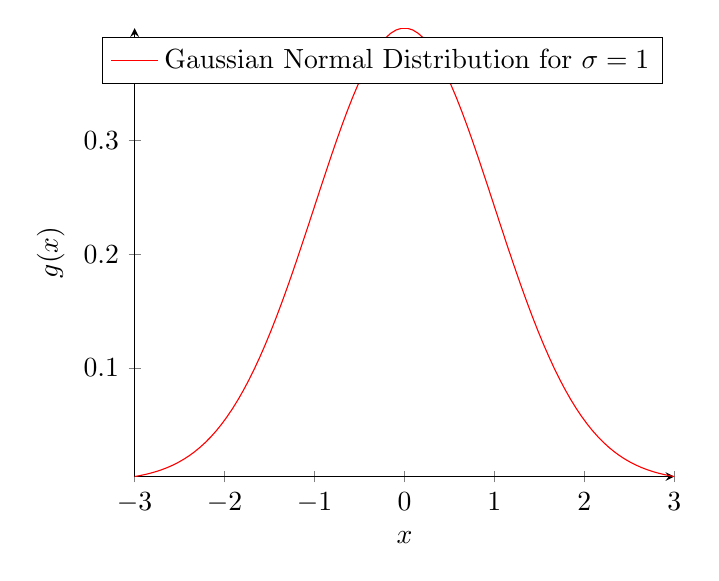
\begin{tikzpicture}
\begin{axis}[
	axis lines = left,
	xlabel = \(x\),
	ylabel = \(g(x)\),
]
\addplot[domain=-3:3,
		samples=100,
		color=red,
]
{1 / ((2 * pi)^0.5) * exp(- ((x^2) / 2))};
\addlegendentry{Gaussian Normal Distribution for \(\sigma = 1\)}
\end{axis}
\end{tikzpicture}

To calculate the Gaussian Filter Response, one needs a Gaussian Kernel with a Window-Size. While in general the gaussian filter has an infinite window size, choosing a fixed window size can approximate the gaussian well. In this discrete case \(\sigma\), the standard deviation of the gaussian, can be approximated with \(N\) the size of the window:
\begin{equation}
\sigma  =\sqrt{\frac{N}{2\pi}}
\end{equation}
With \(\sigma\), the gaussian function for point \(x\) can be calculated as:
\begin{equation}
g(x) = \frac{1}{\sqrt{2\pi}\sigma} * e^{{- \frac{x^2}{2\sigma^2}}}
\end{equation}
Once the gaussian function is calculated for the window, the convolution of the data points with the gaussian kernel is performed ,resulting in smoothed over coefficients of the LID net output. The maximum smoothed coefficient is then chosen and the corresponding language is output, which gave us definite improvements over not smoothing the net output at all. In tcl the relevant code part can be seen in~\ref{lst:tclGauss}, in which we presume the window size to mean the number of points we take into account on both sides of the origin, while normally this number is the window size - 1.
\begin{lstlisting}[label=lst:tclGauss,caption=Gaussian Smoothing Filter as implemented in tcl/tk for the jrtk]
    #Windowsize definition
    set ws 5
    set sigma [expr sqrt($ws/(2*[Pi]))]
    #calculate gauss kernel
    for {set k 0} {$k <= $ws} {incr k} {
        set gauss($k) [expr (1/(sqrt(2*[Pi])*$sigma)) * ([E] ** - (( $k ** 2)/ (2 * $sigma ** 2)))]
    }
    #For each frame
    for {set i 0} { $i < [featureSetLID frameN nnBNF]} {incr i} {
        for {set j 0} {$j < 10} {incr j} {
            set values($j) [lindex [featureSetLID frame nnBNF $i] $j]
            set curValue 0
	         #go from $i - $ws to $i + $ws
            for {set k [expr -$ws]} {$k < $ws} {incr k} {
                #Only use the current value if it actually exists
                if {[expr $i + $k] >= 0 && [expr $i + $k] < [featureSetLID frameN nnBNF]} {
                    set cur [lindex [featureSetLID frame nnBNF [expr $i + $k]] $j]
                    #get correct index for gauss kernel, as we only calculated once above for symmetric function
                    if {$k < 0} {
                        set curIdx [expr -$k]
                    } else {
                        set curIdx $k
                    }
		              #running sum of all previous values in the window convoluted with the gaussian kernel.
                    set curValue [expr $curValue + $cur * [set gauss($curIdx)]]
                }
            }
	         #save the value for current language coefficient
            set values($j) $curValue
        }
        #Find maximum on smoothed values
        set max -1
        set maxID -1
        for {set j 0} {$j < 10} {incr j} {
            if {[set values($j)] > $max} {
                set max [set values($j)]
                set maxID $j
            }
        }
        #Set the output as the Language with Max. coefficient.
        set currentOutput $maxID
    }
\end{lstlisting}


We tried different window sizes of which the result can be seen in Tab.~\ref{tab:eval:gr}. 


\begin{table}[h!]
\label{tab:evalTotal}
\centering
\begin{tabular}{| l | r |}
	\hline
	\textbf{Filter} & \textbf{Overall Error}  \\
	\hline
	 Bare Net & \\
	\hline
	Basic Filter &  \\
	\hline
	Advanced Filter Small & \\
	\hline
	Advanced Filter Big &  \\
	\hline
	English &  \\
	\hline
	\textbf{Overall} &  \\
	\hline
\end{tabular}
\caption{Results of different filtering approaches on the tree-net 6-layer net.}
\end{table}
\section{Lecture Data}
\label{sec:eval:ld}
Of course, all the nets were tested against the lecture data corpus, as this is the closest to an actual possible integration into the KIT's lecture Translator. These results for different net setups are summarized in Tab.~\ref{tab:res:ld_eval}. 

	